%
% File acl2014.tex
%
% Contact: koller@ling.uni-potsdam.de, yusuke@nii.ac.jp
%%
%% Based on the style files for ACL-2013, which were, in turn,
%% Based on the style files for ACL-2012, which were, in turn,
%% based on the style files for ACL-2011, which were, in turn, 
%% based on the style files for ACL-2010, which were, in turn, 
%% based on the style files for ACL-IJCNLP-2009, which were, in turn,
%% based on the style files for EACL-2009 and IJCNLP-2008...

%% Based on the style files for EACL 2006 by 
%%e.agirre@ehu.es or Sergi.Balari@uab.es
%% and that of ACL 08 by Joakim Nivre and Noah Smith

\documentclass[11pt]{article}
\usepackage{acl2014}
\usepackage{times}
\usepackage{url}
\usepackage{latexsym}
\usepackage{graphicx}
\usepackage{qtree}

%\setlength\titlebox{5cm}

% You can expand the titlebox if you need extra space
% to show all the authors. Please do not make the titlebox
% smaller than 5cm (the original size); we will check this
% in the camera-ready version and ask you to change it back.


\title{A* search for shift-reduce constituent parsing}

\author{Thang Le Quang \\
  SoICT - HUST\\
  {\tt lelightwin@gmail.com} \\\And
  Yusuke Miyao \\
  National Informatic Institute\\
  {\tt Yusuke@nii.ac.jp} \\\And
  Hiroshi Noji \\
  National Informatic Institute\\
  {\tt Noji@nii.ac.jp} \\}

\date{}

\begin{document}
\maketitle

\begin{abstract}
	The approach of global discriminative shift-reduce parsing is quite successful, giving 	state-of-the-art performance both for constituency and dependency parsing problem, but most of existing parsers rely on some approximations such as beam search, which discards the optimality. In this paper, we explain how exact search become possible for constituency shift-reduce parsing and explore the effect of optimality empirically. This is the first work on exact search for shift-reduce parsing in a global discriminative setting. The key components of our system are the new feature templates to reduce the time complexity and several A* heuristics for keeping a tractable runtime. Experiments on the standard Penn Treebank verifies the effectiveness of exact search: our new features is not as strong as richer features with the same beam size, but with A* search, it produces F-score of 91.1\% that other beam-based systems cannot reach even with very large beam sizes.
\end{abstract}
\section {Introduction}
Shift-reduce parsing is one of the most classical method for syntactic parsing. In this approach, a parse tree is considered as a set of shift-reduce actions. In all possible parse trees whose scores are the sum of model scores assigned to its shift-reduce actions, the system would select the candidate having the highest score as a result. The approach of shift-reduce parsers is very successful. The advantage of this method is that it can exploit very rich features with a global decoding which leads to very high accuracies. \cite{2006Wang} present the first research on shift-reduce parser which can reach to 88\% F-score on English WSJ tree bank using SVM approach. In \cite{2009Zhang}, they has proposed out the global discriminative training for shift-reduce parsing which can achieve state-of-the-art performance for Chinese constituent parsing with the use of averaged perceptron from \cite{2004Collins}. Utilizing and extending the approach of \cite{2009Zhang}, \cite{2012Zhu} has built a fast and accurate constituent shift-reduce parser which even outperforms the previous state-of-the-art CYK-based parses such as Berkeley parser and Stanford parser.\\
\indent However, there is a problem which is still existed in those shift-reduce parsing system: all of them has to use inexact search to do the work in the decoding process. \cite{2006Wang} uses greedy search performing a deterministic decoder which must sacrifice a large space of candidate parse trees. \cite{2009Zhang} and \cite{2012Zhu} use beam search to extend the candidate space but it still cannot guarantee the exactness. We have a hypothesis that inexact search such as beam and greedy method may cause some searching errors and make the performance become worse than exact search. Therefore, in order to investigate the effect of this search errors, we would like to propose a strategy to perform an exact search for shift-reduce parsing by using A* heuristic. We apply our heuristic into the baseline shift-reduce constituent parsing of \cite{2009Zhang} to test our hypothesis. In our understanding, there is no previous research which can achieve the exactness on global discriminative training for shift-reduce parsing. Our final experiments on WSJ dataset has shown that our parser can overcome the previous constituent shift-reduce parsers in terms of F-score and even gives a comparable accuracy to the state-of-the-art parsers.
\subsection*{Related works}
\cite{2003DanNAACL} has proposed the first research on A* parsing for PCFG model. This system has maintained an agenda to store the processed nodes and extend them in a best-first order by using inside scores and an A* heuristic of outside scores. In their system, Klein and Manning summarized the context to calculate the A* heuristic of the outside probability. Therefore, they have to precomputed and stored the scores of all possible context summaries. They have reported that this heuristic can ignore more than 97\% of total possible nodes and lead the search reaching to goal very fast. However, A* heuristic is very difficult to be applied into the shift-reduce parsers. There are two main challenges in this approach: the first one is the very large search space caused by their rich features. The second one is that the model scores in shift-reduce parsing are always updated overtime due to the incremental training and cannot be directly precomputed as in \cite{2003DanNAACL}. \\
\indent Actually, there are still few parsers which try to perform exact search on shift-reduce parsing. \cite{2010Huang} uses dynamic programming to reduce the total time complexity to polynomial but they still have to use beam search in the decoding process. \cite{2006Sagae} and \cite{2013Zhao} has presented their ways of how to utilize best first search in shift-reduce parsing. However, these two system are locally trained on the maximum entropy model and their performances are still very far behind from the shift-reduce parsing system which has been trained by global discriminative method such as \cite{2012Zhu} or \cite{2009Zhang}. In our system, we firstly build the best first shift-reduce constituent parsing based on the dynamic algorithm of \cite{2010Huang}, and then apply our proposed A* heuristic to make the exact search in the shift-reduce approach become possible for the first time.
\section {Our baseline Shift-Reduce parser} 
In order to achieve our goal, we built a baseline parser which is adapted from \cite{ref:2012Zhu}. Our baseline parsing system follows the shift-reduce process of (Sagae, 2005) and use structured perceptron to obtain the global discriminative training.
\subsection{Shift-Reduce Constituent Parsing}
Shift-reduce parsing can be considered as a state transition system, which means that it includes a set of states and actions. From a current state, each action will create a new corresponding state. A state consists of two data structures: a stack \textit{S} of constructed phrases and a queue \textit{Q} of remain tagged words in the input sentence. Whereas a set of actions in the shift-reduce parsing process includes:
\begin{itemize}
	\item SHIFT: pop the front word from \textit{Q} and push it onto \textit{S}
	\item B-REDUCE-L/R(X): pop the two top nodes from \textit{S} and use the binary rule set to combine them into new constituent node with label X, and push X onto \textit{S}. L means that head of X is its left child, and vice versa with R.
	\item U-REDUCE(X): pop the top constituent off \textit{S}, use the unary rule set to combine them into new constituent node with label X, and push X onto \textit{S}.
	\item FINISH: pop the root node (Sentence) off \textit{S} and end the shift-reduce parsing.
\end{itemize}

The parsing process begins with a start state: empty stack and queue of input tagged sentence and go through a sequence of shift-reduce actions until it perform the FINISH action and reach the final state: an empty stack and an empty queue. Each shift-reduce action has been assigned a score causing that the score of each final state will be sum of the score of all its sequence states. The parsing system will select the parse tree corresponding to the final state with highest accumulative score.

\subsection{Average perceptron training}
As we mentioned above, we used the averaged perceptron algorithm adapted from \cite{ref:2004Collins} to train our model as in \cite{ref:2012Zhu}. For a given input sentence $x$, the initial state has an empty stack and a queue that contains all the input words from the sentence. An beam search strategy will be used to find the candidate final state. Specifically, an agenda is used to keep the k-best states in terms of accumulative score at each step. At initialization, the agenda contains only the initial state. At each step, every states in the agenda are popped out and create a set of new states by applying the shift-reduce actions, and the top k from the newly constructed states are put back onto the agenda. The process repeats until the agenda is empty, and the final state with highest score $F(x)$ is selected as the output. We can call it as a beam search decoder.
\begin{equation}
	F(x) = arg\max_{s \in Beam(x)} Score(s)
\end{equation}

Here $Beam(x)$ is the set of states existed in the beam width of the decoder. The score of a state $s$ is the total score of the shift-reduce actions that have been applied to build the state:
\begin{equation}
	Score(s) = \sum_{i = 0}^{N} \Phi(a_i).\vec{w}
\end{equation}

\begin{table*}[t]
	\begin{center}
		\caption{\label{perceptron} Averaged perceptron algorithm}
		
		\begin{tabular}{|l|l|}
			\hline
			\bf Inputs & Training examples ($x_i,y_i$) \\
			\bf Initialization & $\vec{w}$ = 0 \\
			\bf Output & averaged weights $\vec{w}$ \\
			\hline
			\bf Algorithm 	& For $t = 1 ...T, i = 1 ...n$ \\
			& --- Calculate $F(x_i) = argmax_{y \in Beam(x_i)}Score(y)$ \\
			& --- If $(F(x_i) \neq y_i)$ then $\vec{w} = \vec{w} + \Phi(y_i) - \Phi(z_i)$ \\
			\hline							
		\end{tabular}
	\end{center}
\end{table*}

Here $\Phi(a_i)$ represents the feature vector for the $i^{th}$ action $a_i$ in state $s$. It is computed by applying the feature templates into the context of $a_i$. N is the total number of actions in $s$.
The parser will go through all the example pairs of sentences and golden final states $(x_i, y_i)$ from the training corpus and use the beam search decoder to produce the candidate $F(x_i)$ and update the weights $\vec{w}$ if $F(x_i)$ does not match with $y_i$. The pseudo-code for average perceptron training is shown as in Table \ref{perceptron}

\subsection{Our modified shift-reduce actions}
One of the bottle-neck in shift-reduce constituent is the unary rules problem. Because of these unary rules, the parse trees for the same sentence can have a different numbers of nodes which leads to different numbers of shift-reduce actions. This is an important problem to solve because the inconsistency in the number of shift-reduce actions can make the may lead to inconsistency performance. In \cite{ref:2012Zhu}, they use a padding method which adds the IDLE action in order to extend the sooner completed states. The IDLE action does not change the current state itself, just to keep the number of actions consistency. However, this method creates the redundancy which may increase the number of actions to $4n$ ($n$ is the length of input sentence) and can only guarantee the local consistency in the beam width. With our system, we the following shift-reduce actions to solve the unary rules problem: 
\begin{itemize}
	\item SHIFT: perform the regular shift action.
	\item SHIFT\&U-REDUCE(X): From the current state $A$, perform the regular shift action creating new state $B$. And then perform regular unary reduce action to create new state $C$ with new constituent label $X$. This action returns state $C$.
	\item B-REDUCE(Y): Perform the regular binary reduce action to form the state with new constituent label $Y$.
	\item B-REDUCE(Y)\&U-REDUCE(X): From the current state $A$, perform the regular binary reduce action to create a state $B$ with constituent label $Y$. After that, perform the unary reduce action from $B$ to create a new state $C$ with new constituent label $X$. This action returns state $C$, too.
	\item FINISH: perform the regular finish action.
\end{itemize}

It is clear to see that we had combine the unary reduce actions with shift and binary reduce actions. It means that there is no unary actions anymore and we have only two main types of actions: \textit{shift} or \textit{binary reduce}. This method has two benefits: first, it can guarantee the global consistency, means that the number of shift-reduce actions for each parse tree will always be $2n$. Second, it does not create any redundant states which make the model become sparser. With the number of actions equaling $2n$, the constituent parsing nearly reduces to dependency parsing.

\subsection{Dynamic programming}
In order to achieve the exactness in parsing, dynamic programming is clearly an important problem to exploit the full space of candidates with the time complexity which is within polynomial limitation. \cite{ref:2010Huang} has proposed the way of using dynamic algorithm into shift-reduce dependency parsing which is based on the graph-structured stack  of \cite{ref:1991Tomita} and the classical CYK algorithm. The key of their approach is to merge the shift states (states after shift action) and b-reduce states (states after binary reduce action) together if they are similar. However, due to the unary actions in constituent parsing, the dynamic programming is difficult to implement because the unary states could not be merged with shift states or b-reduce states. Fortunately, with our modified shift-reduce actions, the unary states are not existed which causes the dynamic programming to be easy to implement.

\section{The influence of feature templates on time complexity}
In shift-reduce parsing, the search space will be very large depending on the feature templates we used. Therefore, in this section, we would like to make some evaluation about the time complexity of feature templates and then design a feature template used for exact search in shift-reduce constituent parsing.

\subsection{Evaluation from the baseline feature template}
In \cite{ref:2009Zhang}, they has designed an efficient baseline feature template which is widely used for shift-reduce constituent parsing. The feature template can be viewed as in table \ref{baseline feat} as long as its components and sub-components has been shown in table \ref{baseline comp} and \ref{baseline subcomp}, respectively.

\begin{table*}[t]
	\caption{\label{baseline feat} A table of baseline feature template}
	\begin{center}
		\begin{tabular}{|l|l|}
			\hline 
			Description & Templates  \\ 
			\hline
			1-grams 	& $s_0.t+s_0.c$   ;   $s_0.w+s_0.c$ ; $s_1.t+s_1.c$   ;   $s_1.w+s_1.c$ \\
			& $s_2.t+s_2.c$   ;   $s_2.w+s_2.c$   ;   $s_3.t+s_3.c$   ;   $s_3.w+s_3.c$ \\
			& $q_0.w+q_0.t$   ;   $q_1.w+q_1.c$   ;   $q_2.w+q_2.t$   ;   $q_3.w+q_3.c$ \\
			
			& $s_0l.w+s_0l.c$   ;   $s_0u.w+s_0u.c$   ;   $s_0r.w+s_0r.c$ \\
			& $s_1l.w+s_1l.c$   ;   $s_1u.w+s_1u.c$   ;   $s_1r.w+s_1r.c$ \\
			\hline
			2-grams 	& $s_0.w+s_1.w$   ;   $s_0.w+s_1.c$   ;   $s_0.c+s_1.w$   ;   $s_0.c+s_1.c$ \\
			& $s_0.w+q_0.w$   ;   $s_0.w+q_0.t$   ;   $s_0.c+q_0.w$   ;   $s_0.c+q_0.t$ \\
			& $q_0.w+q_1.w$   ;   $q_0.w+q_1.t$   ;   $q_0.t+q_1.w$   ;   $q_0.t+q_1.t$ \\
			& $s_1.w+q_0.w$   ;   $s_1.w+q_0.t$   ;   $s_1.c+q_0.w$   ;   $s_1.c+q_0.t$ \\
			\hline
			3-grams 	& $s_0.c+s_1.c+s_2.c$   ;   $s_0.w+s_1.c+s_2.c$ ; $s_0.c+s_1.w+s_2.c$   ;   $s_0.c+s_1.c+s_2.w$ \\
			& $s_0.c+s_1.c+q_0.t$   ;   $s_0.w+s_1.c+q_0.t$   ;   $s_0.c+s_1.w+q_0.t$   ;   $s_0.c+s_1.c+q_0.w$ \\
			\hline
		\end{tabular}
	\end{center}
\end{table*}

To evaluate the time complexity of shift-reduce parsing system applying this feature template, we will reply on the observation that the baseline feature has focused on top four nodes in stack $S$ (table \ref{baseline comp}). With each node, we could consider the parsing process as a CYK process. As we know, dynamic algorithm such as CYK can parse an input sentence within $O(n^3.|G|)$ (cubic time) with unlexicalized case and $O(n^5.|G|)$ with lexicalized case. The table \ref{baseline subcomp} has shown that the baseline feature template uses head word as one of its components, so this is the lexicalized case. Therefore, with the combination of four nodes in the lexicalized case, the parsing system which applies the baseline feature must take a very large time complexity about $O((n^5.|G|)^4)=O(n^{20}.|G|^4)$ in the worst case. In general form, if the feature template focuses on top $k$ nodes in stack $S$, then we will have the time complexity $O((n^5*|G|)^k)$ with lexicalized parsing and $O((n^3*|G|)^k)$ with unlexicalized parsing.

\begin{table}[h!]
	\caption{\label{baseline comp} The components which are used in baseline feature template}
	\begin{center}
		\begin{tabular}{|l|l|}
			\hline 
			component & explanation  \\ 
			\hline
			$s_0$ & $1^{th}$ top node in stack $S$ \\
			$s_1$ & $2^{nd}$ top node in stack $S$ \\
			$s_2$ & $3^{rd}$ top node in stack $S$ \\
			$s_3$ & $4^{th}$ top node in stack $S$ \\
			\hline
			$q_0$ & $1^{th}$ word in queue $Q$ \\
			$q_1$ & $2^{th}$ word in queue $Q$ \\
			$q_2$ & $3^{th}$ word in queue $Q$ \\
			$q_3$ & $4^{th}$ word in queue $Q$ \\
			\hline
			$s_0l$ & left child of $s_0$ \\
			$s_0r$ & right child of $s_0$ \\
			$s_0u$ & unary child of $s_0$ \\
			\hline
			$s_1l$ & left child of $s_1$ \\
			$s_1r$ & right child of $s_1$ \\
			$s_1u$ & unary child of $s_1$ \\
			\hline
		\end{tabular}
	\end{center}
\end{table}

Following the result published in \cite{ref:2013Zhao}, the exact search will be possible to perform if we can reduce the time complexity to $O(n^6)$. Comparing this complexity to the general form of time complexity in shift-reduce parsing: $O((n^5*|G|)^k)$ (lexicalized) and $O((n^3*|G|)^k)$ (unlexicalized), we will have $k=1$ (lexicalized) or $k=2$ (unlexicalized). It means that we have two directions to create our own feature template:

\begin{table}[h!]
	\caption{\label{baseline subcomp} The sub-components which are used in baseline feature template}
	\begin{center}
		\begin{tabular}{|l|l|}
			\hline 
			$X.t$ & PoS tag of X's head word \\
			$X.w$ & X's head word \\
			$X.c$ & X's constituent tag \\
			\hline
		\end{tabular}
	\end{center}
\end{table}

\begin{itemize}
	\item $k=1(lexicalized)$: designing a feature template which focuses only on top node in stack $S$ which can use the head word features.
	\item $k=2(unlexicalized)$: designing a feature template which focuses on top two nodes in stack $S$ without the head word features.
\end{itemize}

\subsection{Our simplified feature template}
As we concluded in the previous section, we will have two strategies of creating a feature template for exact search. With the first approach, the feature template will be so small and lack of information so we created our own feature template based on the second one. 

With the second one, the only problem is the lack of head lexical information. Fortunately, there are many studies on unlexicalized constituent parsing which give high parsing accuracy. \cite{ref:2003Dan2} proposed their first research on unlexicalized parsing. This is a theoretically splitting constituent method which can reach 85.77\% F-score. \cite{ref:2007petrov} has proposed out an extension of \cite{ref:2003Dan2} method which splits the grammar automatically to exploit the latent variables and attain the F-score equaling 90.7\%.

\begin{figure*}[t]
	\centering
	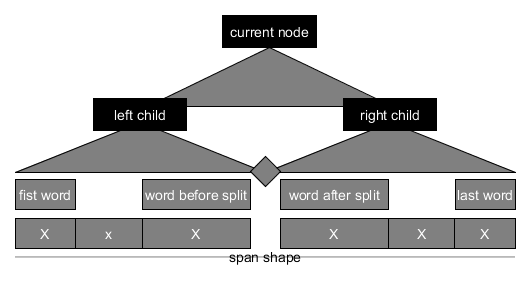
\includegraphics[width=0.7 \textwidth]{spanFeature.png}
	\caption{\label{spanFeature}The span feature from adapted from \cite{ref:2014David}.}
\end{figure*}

\begin{figure}[h!]
	\centering
	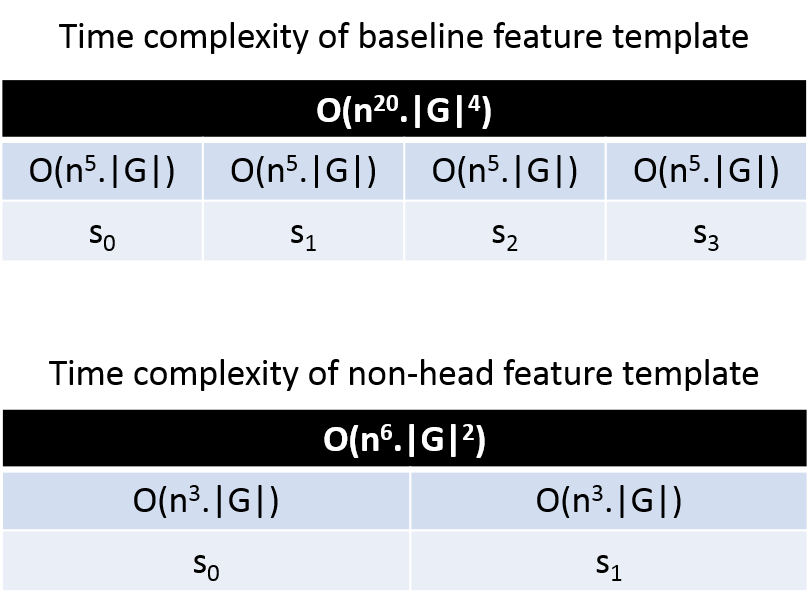
\includegraphics[width=0.45 \textwidth]{FeatureTemplateTimeComplexity.png}
	\caption{\label{featComparison}Comparison of time complexity between baseline and non-head feature template.}
\end{figure}

As in our system, we have designed a feature template which was inspired by the span features in \cite{ref:2014David}. This is a very simple feature set which relied only on the local features within the span of a node and achieve an amazing performace. In the experiment reported in \cite{ref:2014David}, it  has reached an F-score = 89.9\% and outperformed Berkeley parser in terms of parsing many different languages. The span features from this article include the following components for a constituent node (table \ref{simplified subcomp}):
\begin{itemize}
	\item The first and last word of the span of node.
	\item the length of the span of node
	\item The word before and after the split point between left and right child of node.
	\item The shape of word sequence within the span of node (illustrated in figure \ref{spanFeature}):
	\begin{itemize}
		\item X: if the current word's first letter is capital letter.
		\item x: if the current word is normal word.
		\item N: if the current word is a number.
		\item special character such as [' " , .] will remain unchanged.
		\item O: the other cases.
	\end{itemize}
\end{itemize}

\begin{table}
	\caption{\label{simplified subcomp} The sub-components which are used in our simplified feature template}
	\begin{center}
		\begin{tabular}{|l|l|}
			\hline 
			component & explanation \\ 
			\hline
			$X.ft$ &  The first PoS in X's span \\
			$X.fw$ &  The first word in X's span \\
			$X.lt$ &  the last PoS in X's span \\
			$X.lw$ &  the last word in X's span \\
			$X.aSw$ &  The word after-split in X's span \\
			$X.aSt$ &  The PoS after-split in X's span \\
			$X.bSw$ &  The word before-split in X's span \\
			$X.bSt$ &  The PoS before-split in X's span \\
			$X.len$ &  The length of X's span \\
			$X.shape$ &  The shape of X's span \\
			\hline
		\end{tabular}
	\end{center}
\end{table}

Our simplified feature template has been shown in table \ref{simplified feat}. It has focused only on two top nodes in stack $S$($s_0$ and $s_1$) and did not use the head lexical information. Therefore, based on our previous analysis, the time complexity of this feature template will be $O(n^6*|G|^2)$. You can see the illustration of comparison between the baseline and simplified feature template in \ref{featComparison}.

\begin{table*}[t]
	\caption{\label{simplified feat} A table of our simplified feature template}
	\begin{center}
		\begin{tabular}{|l|l|}
			\hline 
			Description & Templates  \\ 
			\hline
			Queue	 	& $q_0.w$+$q_0.t$   ;   $q_1.w$+$q_1.c$   ;   $q_2.w$+$q_2.t$   ;   $q_3.w$+$q_3.c$ \\
			\hline
			$s_0$'s features	 	& $s_0.c$+$s_0.ft$	 ;   $s_0.c$+$s_0.fw$   ;   $s_0.c$+$s_0.lt$   ;   $s_0.c$+$s_0.lw$ \\
			& $s_0.c$+$s_0.aSt$   ;   $s_0.c$+$s_0.aSw$   ;   $s_0.c$+$s_0.bSt$   ;   $s_0.c$+$s_0.bSw$ \\
		    & $s_0.c$+$s_0.ft$+$s_0.lt$   ;   $s_0.c$+$s_0.ft$+$s_0.lw$   ;   $s_0.c$+$s_0.fw$+$s_0.lt$   ;   $s_0.c$+$s_0.fw$+$s_0.lw$ \\
		    & $s_0.c$+$s_0.ft$+$s_0.len$   ;   $s_0.c$+$s_0.fw$+$s_0.len$   ;   $s_0.c$+$s_0.lt$+$s_0.len$   ;   $s_0.c$+$s_0.lw$+$s_0.len$ \\
		    & $s_0.c$+$s_0.ft$+$s_0.lt$+$s_0.len$   ;   $s_0.c$+$s_0.ft$+$s_0.lw$+$s_0.len$ \\
		    & $s_0.c$+$s_0.fw$+$s_0.lt$+$s_0.len$   ;	$s_0.c$+$s_0.fw$+$s_0.lw$+$s_0.len$ \\
			& $s_0.c$+$s_0.len$  ;   $s_0.c$+$s_0.shape$\\
			\hline
			$s_1$'s	features 	& $s_1.c$+$s_1.ft$	 ;   $s_1.c$+$s_1.fw$   ;   $s_1.c$+$s_1.lt$   ;   $s_1.c$+$s_1.lw$ \\
			& $s_1.c$+$s_1.aSt$   ;   $s_1.c$+$s_1.aSw$   ;   $s_1.c$+$s_1.bSt$   ;   $s_1.c$+$s_1.bSw$ \\
			& $s_1.c$+$s_1.ft$+$s_1.lt$   ;   $s_1.c$+$s_1.ft$+$s_1.lw$   ;   $s_1.c$+$s_1.fw$+$s_1.lt$   ;   $s_1.c$+$s_1.fw$+$s_1.lw$ \\
			& $s_1.c$+$s_1.ft$+$s_1.len$   ;   $s_1.c$+$s_1.fw$+$s_1.len$   ;   $s_1.c$+$s_1.lt$+$s_1.len$   ;   $s_1.c$+$s_1.lw$+$s_1.len$ \\
			& $s_1.c$+$s_1.ft$+$s_1.lt$+$s_1.len$   ;   $s_1.c$+$s_1.ft$+$s_1.lw$+$s_1.len$ \\
			& $s_1.c$+$s_1.fw$+$s_1.lt$+$s_1.len$   ;	$s_1.c$+$s_1.fw$+$s_1.lw$+$s_1.len$ \\
			& $s_1.c$+$s_1.len$  ;   $s_1.c$+$s_1.shape$\\
			\hline
		\end{tabular}
	\end{center}
\end{table*}
\section{A* decoder for Shift-Reduce Parsing}
A* search is a very well-known algorithm which belongs to the best-first algorithm. The best-first algorithm uses an agenda to store all the processed points in the searching process. In each step, the most promising point will be used to extend until we reach the final point.\\
\indent However, unlike the regular best first algorithm which uses only the path cost $g(x)$ of each point $x$ in agenda to calculate the best point, A* algorithm also uses an heuristic $h(x)$ which is an admissible heuristic of the path from $x$ to the final point. It means that each point $x$ in A* algorithm will have the score calculated by:

\begin{equation}
	score(x) = g(x)+h(x)
\end{equation}

A* algorithm can guarantee to find the goal with smallest path cost in a shorter time than regular best-first search. To make sure that A* algorithm is efficient, $h(x)$ should satisfy two characters:
\begin{itemize}
	\item admissible: the heuristic must be greater or equal than the real highest cost we have to take in order to get to the final point: $h(x) \geq h_{real}(x)$
	\item consistency: $h(x) \leq d(x,y)+h(y)$, for every ($x,y$) where $y$ is next to $x$, $d(x,y)$ is the cost from $x$ to $y$. This is an additional condition.
\end{itemize}
Therefore, it is plain to see that $h(x)$ is the key of A* algorithm's efficiency.

\subsection{Best first decoder}
In order to utilize A* heuristic, we firstly built our best first decoder which is similar the one in \cite{2013Zhao} but for constituent parsing. Let us denote that $BFS(x)$ is the candidate final state returned by the best first decoder. The best first decoder can be described as follows:
\begin{itemize}
	\item Set up an agenda adding the initial state.
	\item In each step, popping out the best candidate in agenda and extend it by using the shift-reduce actions. After that, put the newly constructed states back into agenda.
	\item Looping until the popped candidate from agenda is the final state.
\end{itemize}

In best first decoder, the model score of each state $s$ is the cost path, the model score of each shift-reduce actions $a_i$ is the transition cost between each state. Let us recall that the model score of state $s$ is the sum of model score of all its shift-reduce actions $a_i$ as in (4). The model score of $a_i$ is calculated as in equation (5). If we use A* decoder, $score(s)$ will be calculated by $g(s)+h(s)$, where $h(s)$ is the heuristic which will be discussed in the next section. The training process of shift-reduce parsing with best first decoder is illustrated in table \ref{best first perceptron}.

\begin{equation}
	score(s) = g(s) = \sum_{i = 0}^{N} score(a_i)
\end{equation}

\begin{equation}
	score(a_i) = \Phi(a_i).\vec{w}
\end{equation}

\begin{table*}[t]
	\begin{center}
		\caption{\label{best first perceptron} Averaged perceptron algorithm with best first search decoder.}
		\begin{tabular}{|l|l|}
			\hline
			\bf Inputs & Training examples ($x_i,y_i$) \\
			\bf Initialization & $\vec{w}$ = 0 \\
			\bf Output & averaged weights $\vec{w}$ \\
			\hline
			\bf Algorithm 	& For $t = 1 ...T, i = 1 ...n$ \\
			& --- Calculate $F(x_i) = BFS(x_i)$ \\
			& --- If $(F(x_i) \neq y_i)$ then $\vec{w} = \vec{w} + \Phi(y_i) - \Phi(z_i)$ \\
			\hline							
		\end{tabular}
	\end{center}
\end{table*}

The only remain bottle-neck is that the negative score problem happened in the shift-reduce parsing process. In best-first search algorithm, the transition of each shift-reduce actions must be positive. However, due to the learning strategy of averaged perceptron, there still exist a negative value in the weights vector $\vec{w}$, and this may lead to negative score problem. Concerning about this problem, we solved this by adding a certain offset value to the transition score of each actions to keep it positive. Because the number of shift-reduce actions is always $2n$ (section 2.3) in our system, the rank of final states is still the same as before. So it will be able to apply this method.

\begin{table*}
	\begin{center}
		\caption{\label{first experiment} The experiment on the development set.}
		\begin{tabular}{|p{2cm}|p{3cm}|p{3cm}|p{3cm}|p{3cm}|}
			\hline 
			System & F-score on BF & parsing speed on BF & F-score on SF & parsing speed on SF \\ \hline
			beam search decoder with $beam = 16$ & 89.07\% & 25 sentences/s & 88.72\% & 30 sentences/s \\ \hline
			beam search decoder with $beam = 32$ & 89.87\% & 10 sentences/s & 89.33\% & 13 sentences/s \\ \hline	
			beam search decoder with $beam = 64$ & 90.3\% & 3.4 sentences/s & 90.15\% & 4.5 sentences/s \\ \hline
			beam search decoder with $beam = 128$ & 90.3\% & 1.05 sentences/s & 90.23\% & 1.36 sentences/s\\ \hline
			$A*$ decoder & N/A & N/A & 90.7\% & 1.2 sentences/s \\
			\hline
		\end{tabular}
	\end{center}
\end{table*}


\subsection{Grammar projection}
\textit{Grammar projection} is an interesting idea published in \cite{2003DanNAACL} and this may be the first research on A* parsing in our knowledge. In this method, they have projected the original grammar rules to a simpler grammar rules. Each projected production rule always have the PCFG probability that is the maximum value of all the original production rules projecting to it. With this conversion, the outside PCFG score of the parse tree constructed by this projected grammar is always greater or equal to the real outside PCFG score and it can be an heuristic for A* search.\\
\indent In our system, we design our own grammar projection based on the filter projection from \cite{2003DanNAACL} with some modification which is suitable with shift-reduce parsing:
\begin{itemize}
	\item project all the complete constituent tags such as [NP, VP, ADJP...] into one single label called [XTAG].
	\item keeping all the incomplete constituent tags such as [NP*, AP*, ADJP*] and the PoS tag as before.
\end{itemize}

Corresponding to this projection, the features will also be projected in our system. The projected features will have the weight equaling the maximum value of all features which project it. For example, there are shift features whose types are $s_0.fw$+$s_0.c$ with values: ([google+VP]; [google+NP]; [google+AP]) with the weights (14.65; 5.67; 8.2), respectively. They will be projected into one value: [google+XTAG] with the weight equaling to 14.65.\\
\indent In our A* decoder, with each state $s$, we will perform the best first search with these projected grammar rules and features to find the heuristic final state $f'$. After projecting, the time complexity of decoding proces will be reduced significantly and can be performed by best first search. The transition score from $s$ to $f'$ will be the heuristic of $s$ in A* search. Because the projected features is the maximum summarization of the original features in terms of weight values, the heuristic transition score will always be greater or equal than the real transition score. It means that the grammar projection heuristic presented here is an \textit{admissible} heuristic.

\subsection{The less constituent heuristic}
The \textit{less constituent} is an heuristic which have been proposed by us based on this observation: if we reduce the number of nodes focused in the feature template, then we can significantly reduce the time complexity. Therefore, if we focused on only $s_0$ instead of both $s_0$ and $s_1$, the time complexity for calculation will be reduced to $O(n^3.|G|)$ which can be decoded by best first search (similar to normal CYK algorithm). As in grammar projection, the heuristic transition score is calculated by best first search after considering less constituent will be the heuristic for A* search. More specifically, to calculate this heuristic, the $s_0$'s features in table \ref{simplified feat} will still be the same but the $s_1$'s features will be ignored and carry the maximum weight value of their types.


For example, the current state $s$ have three attached features: [$s_0.c$+$s_0.ft$], [$s_0.c$+$s_0.fw$] and [$s_1.c$+$s_1.fw$]. Then the two features whose type is [$s_0.c$+$s_0.ft$], [$s_0.c$+$s_0.fw$] will be extracted from $s$ and calculated normally, but the [$s_1.c$+$s_1.fw$] feature of $s$ will be assigned the maximum weight value of all features whose type is [$s_1.c$+$s_1.fw$]. Because the $s_1$'s weights after being ignored are always greater or equal (maximum) than the original $s_1$'s weights, it is clear to see that the heuristic transition score calculated by this way is always greater or equal than the real transition score and this heuristic is also admissible.

\subsection{Our cascaded heuristic}
Both of those two above heuristics have their own problem: calculating the \textit{grammar projection} heuristic will have time complexity = $O(n^6*|g|^2)$ where $g$ is the projected grammar, and calculate the \textit{less constituent} heuristic will have time complexity = $O(n^3*|G|)$. Both of calculation may be a little expensive so we combine them together to reduce the total time complexity. \\
\indent The process of calculating our heuristic could be described as follows: we use the \textit{less constituent} method to calculate A* heuristic for the original best first decoder. And in the process of calculating less constituent heuristic, we use the \textit{grammar projection} to guide the best first search go faster. As you can see, this heuristic is a cascaded type in which an A* heuristic is calculated by another A* heuristic. This method will lead to significant speed-up: the time complexity of calculating \textit{less constituent} will be as fast as the \textit{filter} heuristic in \cite{2003DanNAACL}, and the \textit{less constituent} is also an effective heuristic which will lead the original best first decoder go faster to the best final state.

\begin{figure}[t]
	\centering
	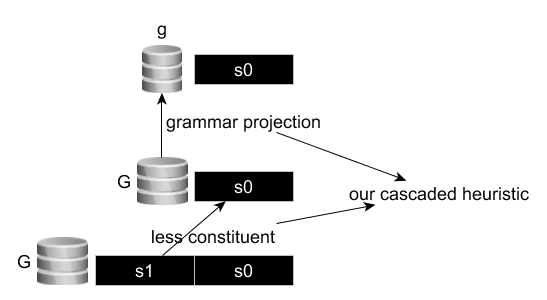
\includegraphics[width=0.5 \textwidth]{cascadedAstar.png}
	\caption{\label{spanFeature}The span feature from adapted from \cite{2014David}.}
\end{figure}
\section{Experiment}
\subsection{Preparation}
We evaluate our A* shift-reduce parser on the Wall Street Journal (WSJ) corpus of the Penn Treebank project with the standard split: sections 2-21 were used for training, section 22 as a development set, and section 23 was used for testing. All our experiments reported in this paper was performed on [our computer configuration].

We used the head finder of \cite{ref:1999Collins} to define the head constituent tag for each phrase in the corpus, and adapted the binarization of \cite{ref:2009Zhang} to binarize our grammar rules. We also used Stanford PoS tagger (with the accuracy = 97\%) to produce the tagged sentence as an input for our shift-reduce constituent parsing. To evaluate the ParseVal F-score, we utilize EVALB program.

\subsection{The experiment results on development set}
On the development set, we make an experiment of comparing our proposal A* decoder with beam search decoder. We also test these decoders in both baseline and simplified feature template. The experiment results can be viewed in table \ref{first experiment}.

\subsection{The experiment results on test set}
On the test set, we make an experiment for comparing our A* parser with the state-of-the-art parsing systems. The results of this experiment are shown in table \ref{second experiment}.
\begin{table}
	\begin{center}
		\caption{\label{second experiment} Results of the final experiment on test set to compare our A* shift reduce parser with other parsing system.}
		\begin{tabular}{|l|l|l|}
			\hline \bf System & \bf F-score \\ \hline
			Johnson and Charniak (2005) & 91.4\% \\
			Mc Closky (2006) & 92.1\%\\
			Collins (1999), Bikel (2004) & 87.7\% \\
			Berkeley Parser & 90.1\%  \\
			Stanford Parser &  90.4\% \\
			SSN parser - Henderson(2004) & 89.4\%  \\
			Zhang Yue - baseline (2012) & 89.8\% \\
			\textbf{This paper} & 91.1\% \\
			\hline
		\end{tabular}
	\end{center}
\end{table}


\section{Discussion}
 	It is clearly to see that inexact search cannot exploit the potential of such feature template like exact one. In the future, we will study how to design a good A* parser (hierarchical A* with reduced-constituent approach) which can apply arbitrary feature sets without taking too much parsing time.

% include your own bib file like this:
%\bibliographystyle{acl}
%\bibliography{acl2014}

\begin{thebibliography}{Reference}

\bibitem[David, 2014]{ref:2014David}
\newblock David Hall, Greg Durrett and Dan Klein. 2014.
\newblock Less Grammar, More Features.
\newblock In Proceedings of the 52nd Annual Meeting of the Association for Computational Linguistics (Volume 1: Long Papers), pages: 228-337, Baltimore, Maryland.
	
\bibitem[Zhao, 2013]{ref:2013Zhao}
\newblock Kai Zhao, Jame Cross and Liang Huang. 2013.
\newblock Optimal Incremental Parsing via Best-First Dynamic Programming.
\newblock In Proceedings of EMNLP 2013.

\bibitem[Zhu, 2012]{ref:2012Zhu}
\newblock Muhua Zhu, Yue Zhang, Wenliang Chen, Min Zhang and Jingbo Zhu. 2013.
\newblock Fast and Accurate Shift-Reduce Constituent Parsing
\newblock In proceedings of ACL 2013. Sophia, Bulgaria. August.
 
\bibitem[Huang, 2010]{ref:2010Huang}
\newblock Liang Huang and Kenji Sagae. 2010. 
\newblock Dynamic programming for linear-time incremental parsing. 
\newblock In Proceedings of ACL 2010.

\bibitem[Zhang, 2009]{ref:2009Zhang}
\newblock Yue Zhang and Stephen Clark. 2009.
\newblock Transition-based parsing of the Chinese Treebank using a global discriminative model.
\newblock In Proceedings of IWPT, Paris, France, October.

\bibitem[Xavier, 2008]{ref:2008Xavier}
\newblock Xavier Carreras, Michael Collins, and Terry Koo. 2008.
\newblock Tag, dynamic programming, and the perceptron for efficient, feature-rich parsing.
\newblock In Proceedings of CoNLL, pages 9-16, Manchester, England.

\bibitem[Huang, 2008]{ref:2008Huang}
\newblock Liang Huang. 2008.
\newblock Forest reranking: discriminative parsing with non-local features.
\newblock In Proceedings of ACL, pages 586-594, Ohio, USA.

\bibitem[Petrov, 2007]{ref:2007petrov}
\newblock Slav Petrov and Dan Klein. 2007.
\newblock Improved inference for unlexicalized parsing.
\newblock In Proceedings of HLT/NAACL, pages 404-411, Rochester, New York, April.

\bibitem[McClosky, 2006]{ref:2006Closky}
\newblock David McClosky, Eugene Charniak, and Mark Johnson. 2006.
\newblock Effective self-training for parsing.
\newblock In Proceedings of the HLT/NAACL, Main Conference, pages 152-159, New York City, USA, June.

\bibitem[Sagae, 2006]{ref:2006Sagae}
\newblock Kenji Sagae and Alon Lavie. 2006.
\newblock A best-first probabilistic shift-reduce parser
\newblock In Proceedings of the COLING/ACL, Main Conference, poster sessions, pages 691-698

\bibitem[Charniak, 2005]{ref:2005Charniak}
\newblock Eugune Charniak and Mark Johnson. 2005.
\newblock Coarse-to-fine n-best parsing and maxent discriminative reranking.
\newblock In Proceeding of ACL, pages 173-180.

\bibitem[Henderson, 2004]{ref:2004Henderson}
\newblock James Henderson. 2004.
\newblock Discriminative training of a neural network statistical parser.
\newblock In Proceedings of ACL.

\bibitem[Collins, 2004]{ref:2004Collins}
\newblock Michael Collins and Brian Roark. 2004.
\newblock Incremental parsing with the perceptron algorithm.
\newblock In Proceedings of ACL, Stroudsburg, PA, USA.

\bibitem[Taskar, 2004]{ref:2004Taskar}
\newblock Ben Taskar, Dan Klein, Michael Collins, Daphne Koller, and Chris Manning. 2004.
\newblock Max-margin parsing.
\newblock In Proceedings of EMNLP.

\bibitem[Dan2, 2003]{ref:2003Dan2}
\newblock Dan Klein and Christopher D Manning. 2003. 
\newblock Accurate Unlexicalized Parsing  
\newblock In Proceedings of ACL 2003.

\bibitem[Dan1, 2003]{ref:2003Dan1}
\newblock Dan Klein and Christopher D Manning. 2003. 
\newblock A* parsing: Fast exact Viterbi parse selection. 
\newblock In Proceedings of HLT-NAACL.

\bibitem[Collins, 2000]{ref:2000Collins}
\newblock Michael Collins. 2000.
\newblock Discriminative reranking for natural language processing.
\newblock In Proceedings of ICML, pages 175–182, Stanford, CA, USA.

\bibitem[Collins, 1999]{ref:1999Collins}
\newblock Michael Collins. 1999.
\newblock Head-driven statistical models for natural language parsing. 
\newblock Ph.D. thesis, University of Pennsylvania.

\bibitem[Collins, 1997]{ref:1997Collins}
\newblock Michael Collins. 1997.
\newblock Three generative, lexicalised models for statistical parsing. 
\newblock In Proceedings of ACL, Madrid, Spain.
 
\bibitem[Tomita, 1991] {ref:1991Tomita}
\newblock Masaru Tomita. 1991.
\newblock Generalized LR Parsing.
\newblock Kluwer Academic Publishers.

\end{thebibliography}

\end{document}
